\documentclass[french]{hermes-journal}

\ria{2014}{28}{2-3}

\usepackage{textcomp}

%\usepackage{lmodern}
\usepackage{fontspec}%% load unicode fonts for xelatex

%\DeclareUnicodeCharacter{00A0}{~}
%\DeclareUnicodeCharacter{00DF}{\ss}
%\DeclareUnicodeCharacter{00E4}{\"a}

% pagination
\firstpagenumber{1}

\newcommand*{\lpath}{./}
%\usepackage[cmex10]{amsmath, mathtools}
%\usepackage{amsmath,amssymb,amsbsy,amsfonts,amsthm}
%\usepackage[ruled,vlined]{algorithm2e}
\usepackage{amsmath,amssymb,amsbsy,amsfonts}
\usepackage{mathtools}
\usepackage{booktabs}
\usepackage{multirow}
\usepackage{bm}
\usepackage{enumerate}
\usepackage{url}
\usepackage{fancyvrb}
\usepackage{yfonts}
\usepackage{wrapfig}
\usepackage{subfigure}
\usepackage{tikz}
\usetikzlibrary{bayesnet}
\newcommand{\tikzmark}[1]{\tikz[overlay,remember picture] \node (#1) {};}
\usepackage{calc}%    For the \widthof macro
\usepackage{xparse}%  For \NewDocumentCommand
\usepackage{adjustbox}


%% Variable de compilation
\newif\ifbeamer
\beamerfalse
\newcommand{\beamer}[2]{\ifbeamer #1 \else #2 \fi}
%%%

%\usepackage[latin1]{inputenc}
\usepackage[utf8]{inputenc} % manage utf8 encodage 
%\usepackage[english]{babel} % for french document ! dirty enumerate style,+ bad change rectangle colors for section linking.
\usepackage{fancyhdr} % for heading
\usepackage{listings}
\usepackage[colorlinks=true, urlcolor=blue]{hyperref} % url, link
\usepackage{graphicx}
\usepackage{geometry}

%\usepackage[cmex10]{amsmath, mathtools}
\usepackage{amsmath,amssymb,amsbsy,amsfonts,amsthm}
\usepackage{multirow}
\usepackage{bm}
\usepackage{enumerate}
\usepackage{url}
\usepackage[ruled,vlined]{algorithm2e}
\usepackage{fancyvrb}
\usepackage{yfonts}

\usepackage{wrapfig}
\usepackage{tikz}
    %\input{../tikz.conf}
    
\usetikzlibrary{bayesnet}
    
%%%%%%%%%%% Box 
\usepackage{calc}%    For the \widthof macro
\usepackage{xparse}%  For \NewDocumentCommand
\newcommand{\tikzmark}[1]{\tikz[overlay,remember picture] \node (#1) {};}

%%%%%%%%%% Math
\renewcommand{\text}{\textnormal}
\newcommand{\pr}{\mathbf{p}}
\newcommand{\E}{\mathbb{E}}
\newcommand{\divkk}{\mathbb{K}}
\newcommand{\entropy}{\mathbb{H}}
\newcommand{\gem}{\mathrm{GEM}}
\newcommand{\Mult}{\mathrm{Mult}}
\newcommand{\DP}{\mathrm{DP}}
\newcommand{\IBP}{\mathrm{IBP}}
\newcommand{\M}{\mathcal{M}}
\newcommand{\V}{\mathcal{V}}
\newcommand{\N}{\mathcal{N}}
    
\makeatletter
\NewDocumentCommand{\DrawBox}{s O{}}{%
    \tikz[overlay,remember picture]{
    	\IfBooleanTF{#1}{%
    		\coordinate (RightPoint) at ($(left |- right)+(\linewidth-\labelsep-\labelwidth,0.0)$);
    	}{%
    	\coordinate (RightPoint) at (right.east);
    }%
    \draw[red,#2]
    ($(left)+(-0.2em,0.9em)$) rectangle
    ($(RightPoint)+(0.2em,-0.3em)$);}
}

\NewDocumentCommand{\DrawBoxWide}{s O{}}{%
	\tikz[overlay,remember picture]{
		\IfBooleanTF{#1}{%
			\coordinate (RightPoint) at ($(left |- right)+(\linewidth-\labelsep-\labelwidth,0.0)$);
		}{%
		\coordinate (RightPoint) at (right.east);
	}%
	\draw[red,#2]
	($(left)+(-\labelwidth,0.9em)$) rectangle
	($(RightPoint)+(0.2em,-0.3em)$);}
}
\makeatother
%%%%% ! Box

\geometry{
      a4paper,
	    body={160mm,260mm},
	    left=25mm,top=20mm,
	    headheight=4mm,headsep=8mm,
        footskip=10mm,
        }
                                              

%%%%%%%%%%%%%%%%%%%%%%%%%%%%%%%%%%%%%%%%%%%%%%%%%%%%%%%%%%%%%%%%%%%%%%%%%%%%%%%%%%%%%%%%%%%%%%%%%%%%%%
%%%%% => Internal
%%%%%%%%%%%%%%%%%%%%%%%%%%%%%%%%%%%%%%%%%%%%%%%%%%%%%%%%%%%%%%%%%%%%%%%%%%%%%%%%%%%%%%%%%%%%%%%%%%%%%%

% itemize item def
%% \begin{itemize}\itemsep2pt % example space betwew item
%\renewcommand{\FrenchLabelItem}{\textbullet}
\renewcommand{\labelitemi}{$\bullet$}
\renewcommand{\labelitemii}{$\cdot$}
\renewcommand{\labelitemiii}{$\diamond$}
\renewcommand{\labelitemiv}{$\ast$}

% equation reference
\renewcommand{\theequation}{\thesection.\arabic{equation}}

%%%%%%%%%%%%%%%%%%%%%%%%%%%%%%%%%%%%%%%%%%%%%%%%%%%%%%%%%%%%%%%%%%%%%%%%%%%%%%%%%%%%%%%%%%%%%%%%%%%%%%
%%%%% => Alias
%%%%%%%%%%%%%%%%%%%%%%%%%%%%%%%%%%%%%%%%%%%%%%%%%%%%%%%%%%%%%%%%%%%%%%%%%%%%%%%%%%%%%%%%%%%%%%%%%%%%%%

% write code
\lstnewenvironment{C}[1]
{\lstset{language=C,
      frame=tBRl,
      basicstyle=\scriptsize,stringstyle=\emph,showstringspaces=false,
      numbers=left,numberstyle=\tiny,
      breaklines=true, columns=flexible, title={#1}}
}{}
      
%%%%%%%%%%%%%%%%%%%%%%%%%%%%%%%%%%%%%%%%%%%%%%%%%%%%%%%%%%%%%%%%%%%%%%%%%%%%%%%%%%%%%%%%%%%%%%%%%%%%%%
%%%%% => Preambles Pages
%%%%%%%%%%%%%%%%%%%%%%%%%%%%%%%%%%%%%%%%%%%%%%%%%%%%%%%%%%%%%%%%%%%%%%%%%%%%%%%%%%%%%%%%%%%%%%%%%%%%%%

\pagestyle{fancy}
\fancyhf{} % remove default headers
\fancyfoot[C]{\thepage}
\renewcommand{\footrulewidth}{0.3pt}
\renewcommand{\headrulewidth}{0.3pt}

%%%%%%%%%% Math
\renewcommand{\text}{\textnormal}
\newcommand{\ilfm}{\texttt{ILFM}}
\newcommand{\immsb}{\texttt{IMMSB}}
\newcommand{\mmm}{\texttt{Mixed-Membership}~}
\newcommand{\pr}{p}
\newcommand{\p}{p}
\newcommand{\E}{\mathbb{E}}
\newcommand{\divkk}{\mathbb{K}}
\newcommand{\entropy}{\mathbb{H}}
\newcommand{\gem}{\mathrm{GEM}}
\newcommand{\Mult}{\mathrm{Mult}}
\newcommand{\DP}{\mathrm{DP}}
\newcommand{\IBP}{\mathrm{IBP}}
\newcommand{\M}{\mathcal{M}}
\newcommand{\V}{\mathcal{V}}
\newcommand{\N}{\mathcal{N}}
\newcommand{\mat}[1]{\bm{#1}}
\newcommand{\unit}{1\!\!1}

%\newtheorem{definition}{Definition}[section]
%\newtheorem{proposition}{Proposition}[section]
%\newtheorem{theorem}{Theorem}[section]
%\newtheorem{corollary}{Corollary}[section]


%\title[short header title]{title}
\title[]{Une Etude des Modèles Mixed-Membership pour la Prédiction de Liens dans les Réseaux Sociaux}

%\author[1]{Adrien}{Dulac}
%\author[2]{first name 2}{last name 2}
%
%% addresses are automatically numbered
%\address{...\\...\\
%         ..., country}
%        {e-mail 1}
%\address{...\\...\\
%         ..., country}
%        {e-mail 1}

%\author{\IEEEauthorblockN{Adrien Dulac\IEEEauthorrefmark{1}, Eric Gaussier\IEEEauthorrefmark{1} and Christine Largeron \IEEEauthorrefmark{2}}\\
%\IEEEauthorblockA{\IEEEauthorrefmark{1}
%Univ. Grenoble Alpes, CNRS, Grenoble INP, LIG - F-38000 Grenoble\\
%Email: \{adrien.dulac, eric.gaussier\}@imag.fr}
%\IEEEauthorblockA{\IEEEauthorrefmark{2}
%Univ Lyon, UJM-Saint-Etienne, CNRS, Institut d'Optique Graduate School,\\
%Laboratoire Hubert Curien UMR 5516, F-42023, SAINT-ETIENNE, France\\ 
%Email: christine.largeron@univ-st-etienne.fr}}

\abstract{We assess here whether standard stochastic mixed membership models are adapted for link prediction in social networks by studying how they handle homophily and preferential attachment. To study these properties, we first introduce formal definitions of these phenomena; we then study how stochastic mixed membership models relate to these definitions. Our theoretical analysis reveals that standard stochastic mixed membership models comply with homophily with the similarity that underlies them. For preferential attachment, the situation is more contrasted: if these models do not comply with global preferential attachment, their compliance to local preferential attachment depends on whether the memberships to latent factors are hard or soft, and in the latter case on whether the underlying latent factor distribution is bursty or not. We illustrate these elements on synthetic and real networks by using the generative properties of Bayesian model.}

\resume{Nous évaluons dans ce papier si la classe de modèles, dit mixed-membership, est adaptée pour la prédiction de liens dans les réseaux sociaux en étudiant les comportements de ces modèles vis-à-vis de l'homophilie et de l'attachement préférentiel. Nous introduisons les définitions de ces phénomènes, puis analysons le comportement de  ces modèles. Notre étude théorique révèle que les modèles mixed-membership satisfont l'homophilie avec la similarité naturelle qui les sous-tend. Pour l'attachement préférentiel la situation est plus contrastée: ces modèles ne satisfont pas l'attachement préférentiel global. En revanche, le respect de l'attachement préférentiel local est possible selon que l'appartenance aux classes latentes est stricte ou partielle et, dans ce dernier cas si la distribution sur les classes latentes est bursty ou pas. Nous illustrons ces résultats par des expérimentations réalisés sur des réseaux réels et synthétiques.}

\keywords{Hierachical baysian Models, Random Graph, Machine Learning, Social Networks}

\motscles{Modèle Bayesian Hérarchique, Graphe aléatoire, Apprentissage Automatique, Réseaux Sociaux}


%
%
%
%  Is better abstract ?
%
%
%\significancestatement{We introduce formal definitions of the compliance of probabilistic link prediction models to homophily and preferential attachment in social networks, and show that standard stochastic mixed membership models comply with homophily with the similarity that underlies them. For preferential attachment, the situation is more contrasted: if these models do not comply with global preferential attachment, their compliance to local preferential attachment depends on whether the memberships to latent factors are hard or soft, and in the latter case on whether the underlying latent factor distribution is bursty or not.}


\begin{document}

\maketitle

\newpage






\section{Introduction}

\label{sec:intro}

Plusieurs modèles de prédiction de liens puissants ont été proposés dans la littérature pour apporter une solution au problème dit de \textit{prédiction de liens} consistant à prédire la probabilité d'une relation entre deux n\oe{}uds quelconques dans un réseau social \cite{LibenNowell07, HassanZaki11}.
Parmi ces modèles, la classe des modèles \mmm a reçu une attention particulière due à leur capacité à faire émerger la structure d'un réseau et à inférer des liens non observés.
Deux instances principales de cette classe ont été proposées et étudiées  dans la littérature : le modèle à composition mixte de bloc (MMSB) \cite{MMSB} et son extension non-paramétrique \cite{iMMSB, fan2015dynamic} d'un côté et le modèle à attributs latents (ILFM) \cite{BMF} et son extension non-paramétrique \cite{ILFRM} de l'autre. 


Les modèles probabilistes, tels que ceux considérés sont usuellement évalués empiriquement. Néanmoins, les réseaux sociaux réels exhibent des propriétés générales qui permettent de les caractériser. Dans cette étude, nous traitons deux propriétés importantes, \textit{l'homophilie} et \textit{l'attachement préférentiel} \cite{ Barabasi2003}. Nous étudions dans quelle mesure les modèles de prédiction de liens, de la classe mentionnée, s'y conforment.

L'homophilie est une propriété selon laquelle la probabilité que deux n\oe{}uds du réseau soient liés augmente avec leurs similarités et qui est communément suggérer par la locution \emph{"qui se ressemble s'assemble"}.

L'attachement préférentiel est une propriété "topologique" dans le sens où elle ne dépend que du nombre de connections présentes dans le réseaux. Elle signifie que la probabilité de créer un lien avec un autre n\oe{}ud dépend du nombre de liens de ce dernier (son degré). Cette propriété traduit l'aphorisme populaire \emph{"On ne prête qu'aux riches"}. En théorie des graphes l'attachement préférentiel est évoqué pour expliquer l'émergence de graphes dits "scale-free" qui sont caractérisés par une distribution des degrés en loi de puissance.

L'intérêt de ces propriétés dans l'analyse des réseaux sociaux a été largement mis en avant pour la modélisation de réseaux et l'amélioration des tâches de prédiction de liens comme de détection de communautés.


\section{Modèles de prédictions de liens stochastique}

Les modèles \mmm sont des modèles génératifs basés sur des facteurs latents (aussi appelés classe latentes ou caractéristiques latentes) qui représentent les propriétés, a priori, des n\oe{}uds du graphe $G=(V,E)$ associé au réseau social (chaque n\oe{}ud représente un individu). Nous notons la matrice d'adjacence induite $Y=(y_{ij})_{i,j\in V}$ où $y_{ij}=1$ si un lien est observé entre $i$ et $j$ et $y_{ij}=0$ si un non-lien est observé. Nous dénotons $N$ le nombre de n\oe{}uds du graphe ($N=|V|$). Les modèles \mmm sont caractérisés par le fait qu'un n\oe{}ud peut appartenir à plusieurs facteurs latents. Par exemple, cela peut permettre de modéliser le fait qu'un individu puisse appartenir à plusieurs communautés \footnote{Comme mentionné dans \cite{goldenberg2010survey} }. L'appartenance d'un n\oe{}ud $i$ est encodé dans son facteur latent par un vecteur $\mat{f}_i$ de dimension finie $K$ dans les versions standard des modèles, et de dimension potentiellement infinie dans les versions non-paramétriques, et cette dimension devient un paramètre du modèle. La collection des vecteurs $\mat{f}_{i}$ ($1 \le i \le N$) constitue la matrice de caractéristiques latentes $\mat{F}$. De plus, une matrice de poids $\mat{\Phi}$ est utilisée pour encoder les corrélations entre les caractéristiques latentes. Comme nous travaillons sur des réseaux binaires, les observations (liens) ont pour vraisemblance une distribution de Bernoulli.

Les modèles de la classe des \mmm diffèrent dans la manière dont les matrices $\mat{F}$ et $\mat{\Phi}$ sont générées. Afin de rester dans un cadre le plus général possible, nous considérons ici les versions non-paramétriques du modèle de caractéristiques latentes \cite{ILFRM}, dénoté \ilfm, et du modèle de composition mixte bloc  \cite{iMMSB,fan2015dynamic}, dénoté \immsb. Cela conduit à un nombre de facteurs latents dynamique qui permet à la dimension du modèle de s'adapter à la complexité des données. En pratique, cela est réalisé par l'utilisation de prior non-paramétrique, le processus de Dirichlet Hiérarchique (HDP) pour \immsb\ et le processus du Buffet Indien (IBP) pour \ilfm.~\\

Concernant \ilfm, chaque n\oe{}ud du réseau est représenté par un vecteur de caractéristiques binaires. La probabilité de créer un lien entre deux n\oe{}uds dépend alors uniquement de la matrice de caractéristiques latentes et de la matrice  de poids, où chaque entrée est générée par une distribution normale. La matrice de caractéristiques est générée via un IBP, conduisant à un nombre de caractéristiques théoriquement infini, bien que pour un nombre fini d'observations (de liens), seulement un nombre fini de caractéristiques sont actives. Le processus génératif se résume ainsi :
\begin{enumerate}
\item Génération d'une matrice de caractéristiques $\mat{F}_{N \times \infty}$ : $\mat{F} \sim \IBP(\alpha)$
\item Génération d'une matrice de poids : $\mat{\phi}_{mn} \sim N(0, \sigma_w), \, m,n \in \mathbb{N}^{+*}$
\item Génération d'un lien (ou non lien) pour chaque couple de n\oe{}uds $(i,j)$ : 
\begin{equation*}
y_{ij} \sim \mathrm{Bern}(\sigma(\mat{f}_{i} \mat{\Phi} \mat{f}_{j}^\top))
\label{eq:link-ilfm}
\end{equation*}
\end{enumerate}
%

Où $\top$ représente la transposée et $\sigma$ la fonction sigmoïde permettant de passer d'un ensemble $[-\infty, +\infty]$ vers un ensemble de probabilité $[0,1]$.  $\mat{f}_{i}$ dénote la i-ème ligne de la matrice $F$ comme le vecteur de caractéristiques latent du n\oe{}ud $i$. Finalement, ce modèle définit deux hyper-paramètres, l'un étant le paramètre de concentration $\alpha$ de IPB, et l'autre celui de la variance de la distribution normale des poids $\sigma_w$. \footnote{Dans le cas d'un réseau dirigé, les matrices $\mat{Y}$ et $\mat{\Phi}$ sont symétriques et uniquement leurs parties diagonales supérieures ou inférieures) sont générées}. ~\\


Le modèle \immsb~ quant à lui, génère les distributions d'appartenance aux classes latentes à partir d'un processus (hiérarchique) de Dirichlet. Après quoi, une appartenance à une classe latente par n\oe{}ud est tirée pour chaque couple de n\oe{}uds. Finalement, la probabilité de connecter deux liens est tirée en fonction du poids encodant la corrélation entre ces deux classes, se résumant au processus génératif suivant :
\begin{enumerate}
\item Génération des distributions des classes d'appartenances $\mat{F}_{N \times \infty}$:
   \begin{align}
       \bm{\beta} &\sim \gem(\gamma) \nonumber \\
    \mat{f}_i &\sim \DP(\alpha_0, \beta) \quad\text{ for }  i \in \{1, .., N\} \nonumber
   \end{align}  Où $\gem$ dénote le processus Stick-Breaking qui est une distribution sur la ligne réelle et $\DP$ un processus de Dirichlet \cite{HDP}.
\item Génération de la matrice de poids depuis une distribution Beta :\\
\[ \phi_{mn} \sim \mathrm{Beta}(\lambda_0,\lambda_1), \, m,n \in \mathbb{N}^{+} \]
\item Génération de classes d'appartenance pour la dyade pour chaque couple de n\oe{}uds $(i,j)$ tirés d'une loi multinomiale et génération d'un lien (ou non-lien) : 
   \begin{align}
       z_{i \rightarrow j} \sim&\ \mbox{Cat}(\mat{f}_i) \quad z_{i \leftarrow j} \sim \mbox{Cat}(\mat{f}_j) \nonumber \\
       y_{ij} &\sim \mathrm{Bern}(\phi_{z_{i \rightarrow j}z_{i \leftarrow j}}) \nonumber
    \label{eq:link-immsb}
   \end{align}
\end{enumerate}


Ce modèle contient quatre hyper-paramètres, $(\gamma, \alpha_0)$ pour le HDP et $(\lambda_0, \lambda_1)$ pour la distribution des poids. \footnote{La remarque précèdente concernant les réseaux dirigés s'applique ici aussi.}

Dans l'usage classique des modèles décrits pour la prédiction de liens, des observations (liens) sont disponibles et sont utilisées pour estimer  $\mat{F}$ et $\mat{\Phi}$, à partir desquels de nouveaux liens peuvent être prédits. Dans la suite de ce papier, nous dénoterons par $\mat{\hat{F}}$ et $\mat{\hat{\Phi}}$ les estimations (ie paramètres inférés) de $\mat{F}$ et $\mat{\Phi}$, qui peuvent être obtenues à partir d'algorithmes d'inférence approximés tels que le (collapsed) Gibbs sampling et Metropolis-Hastings ou encore à l'aide d'inférence variationnelle Nous ne les détaillons pas ici et renvoyons le lecteur intéressé à \cite{ILFRM,IBP,HDP,fan2015dynamic}.

Nous dénoterons aussi $\mathcal{M}_e$ la version des deux modèles \ilfm\ and \immsb\ dans lesquels $\mat{F}$ and $\mat{\Phi}$ sont assumés connus et fixés à $\mat{\hat{F}}$ et  $\mat{\hat{\Phi}}$.

La section suivante est consacrée à l'analyse  de ces propriétés pour les modèles \mmm, à savoir, a partir des paramètres appris $\mat{\hat{F}}$ and $\mat{\hat{\Phi}}$.


\section{Homophilie: \emph{"Birds of a feather flock together"}}
\label{sec:homophily}

L'homophilie réfère à la tendance des individus à se connecter à d'autres avec qui ils partagent certaines caractéristiques telles que un statut, des préférences ou intérêts\cite{mcpherson2001birds,lazarsfeld1954friendship}.   Une notion proche est celle d'\emph{assortativité}, qui est plus générale et s'applique à tous types de réseaux, pas seulement sociaux, et qui renvoit à la tendance à se connecter à des individus similaires.


Une définition de l'homophilie a été proposée par \cite{la2010randomization}. Cependant, cette définition considère une seule caractéristique (ie l'âge ou le genre), et ne peut donc pas s'appliquer dans le cadre de modèles \mmm. Nous proposons donc de définir l'homophile comme suit : 
\begin{definition}[Homophilie] \label{def:homophily}
    Suppose $\mathcal{M}_e$ est un modèle de prédiction de liens et $s$ une mesure de similarité entre n\oe{}uds. Nous disons que $\mathcal{M}_e$ est homophilique avec une similarité $s$ ssi, $\forall (i,j,i',j') \in V^4$:
\begin{equation}
s(i,j) > s(i',j')  \implies \pr(y_{ij}=1 \mid \mathcal{M}_e) > \pr(y_{i'j'}=1  \mid \mathcal{M}_e) \nonumber
\end{equation}

\end{definition}

\noindent Cette définition capture directement l'effet \emph{"plus deux n\oe{}uds sont similaires, plus ils ont une chance de se connecter"}. 

Différentes similarités peuvent être considérées, tant qu'elles sont basées sur la mesure des propriétés des n\oe{}uds considérés. Dans les modèles \mmm, ces propriétés ne sont pas directement observées, et sont encodées dans les caractéristique latentes. D'après les paramètres des modèles, nous défissons la notion de similarité naturelle comme étant $s_n(i,j) = \mat{\hat{f}}_{i} \mat{\hat{\Phi}} \mat{\hat{f}}_j^\top$.


On peut voir que \ilfm~  et \immsb, dans le contexte $\mathcal{M}_e$ sont homophiliques avec le respect de $s_n$. En effet, $\pr(y_{ij}=1 \mid \mathcal{M}_e)$ augmente avec $s_n$  pour  \ilfm\ comme la fonction sigmoïde est strictement croissante. De plus, en marginalisant sur les paramètres $z$ dans \immsb\ on a :
\begin{align}
    \pr(y_{ij} =1 \mid \mathcal{M}_e) & = \sum_{k,k'} \pr(y_{ij}=1|\mathcal{M}_e) \pr(z_{i \rightarrow j}=k | \mathcal{M}_e) \pr(z_{i \leftarrow j}=k' | \mathcal{M}_e) \nonumber \\
& = \sum_{k,k'} \hat{\phi}_{k,k'} \hat{f}_{ik} \hat{f}_{jk'} = \mat{\hat{f}}_{i} \mat{\hat{\Phi}} \mat{\hat{f}}_j^\top \nonumber
\end{align}


Nous définissons une seconde similarité, uniquement dépendante des caractéristiques latentes et où la matrice des poids est abandonnée, par $s_l(i,j) = \mat{\hat{f}}_{i} \mat{\hat{f}}_j^\top$. Avec cette similarité, ni \ilfm~ ni \immsb~ sont homophiliques. En effet, supposons que $\mat{\hat{\Phi}}$ est presque nul sur la diagonale, et strictement positive par ailleurs (ce qui est possible pour les deux modèles). Pour \immsb~ on a :
\begin{align*} 
\pr(y_{ij}=1 \mid \M_e) & = \sum_{k' \neq k} \hat{f}_{ik} \hat{\phi}_{kk'} \hat{f}_{jk'}
\end{align*}


comme $\hat{\phi}_{kk} = 0$.  Supposons à présent que : $\mat{\hat{f}}_i=\mat{\hat{f}}_j=(0,1,0)$ et $\mat{\hat{f}}_{i'}=(0.5,0,0.5)$ et $\mat{\hat{f}}_{j'}=(0,1,0)$, alors, $s_l(i,j)=1$ et $s_l(i',j')=0$. Ainsi $\pr(y_{ij}=1 \mid \M_e) = 0$ alors que $\pr(y_{i'j'}=1 \mid \M_e) > 0$. Donc \immsb~ n'est pas homophilique avec $s_l$. De la même manière, en remplaçant $\mat{\hat{f}}_{i'}=(0.5,0,0. 5)$ par $\mat{\hat{f}}_{i'}=(1,0,1)$, on voit que \ilfm~ n'est pas homophilique non plus avec $s_l$.

Cela montre que, pour qu'un modèle soit homophilique, il doit être conçu en fonction de la similarité à la base de la proximité entre individus. \ilfm~ et \immsb~ ont été conçus sur la base de la similarité naturelle qui constitue le paramètre de la distribution de Bernoulli sur les liens. Il est donc trivialement vrai que les modèles soient homophiliques avec $s_n$. Il est néanmoins possible de rendre les modèles homophiliques avec $s_l$ en adaptant le prior sur la matrice $\mat{\Phi}$; par exemple, une matrice de poids diagonale avec des poids constants conduira à des modèles homophiliques. Dans ce cas, les caractéristiques latentes peuvent être interprétées comme des communautés. C'est ce qui est réalisé dans les travaux de \cite{AMMSB} afin de détecter des communautés recouvrantes dans des réseaux sociaux.

\section{Attachement Préférentiel: \emph{"The rich get richer"}}
\label{sec:burstiness}


L'attachement préférentiel est une propriété d'un réseau selon laquelle la probabilité qu'un n\oe{}ud crée un lien avec un autre augmente avec le nombre de liens déja établis par ce dernier (son degré). Cette propriété est lié à un phénomène plus général appelé \textit{burstiness} \footnote{A.L. Barab\'asi, par exemple, utilise ce terme \textit{attachement préférentiel} in \cite{barabasi1999emergence}, et \textit{burstiness} dans \cite{barabasi_burst}.} qui décrit le fait que certains évènements apparaissent en "rafale", c'est à dire qu'une fois qu'ils apparaissent ils ont plus de chance d'apparaître encore. La burstiness a été étudiée dans différents domaines, notamment en traitement automatique du langage et en recherche d'information afin de caractériser l'occurrence des mots \cite{church1995poisson}. Des définitions simples du burstiness ont été proposées \cite{clinchant2008bnb,clinchant2010information}, pour les distributions continues et discrètes, qui capturent le fait que la probabilité de nouvelles occurrences d'un évènement augmente avec le nombre d'occurrences de cet évènement. Nous adaptons ici ces définitions pour l'attachement préférentiel dans les réseaux. De plus, le phénomène peut apparaître à différent niveaux du réseaux : (a) l'attachement préférentiel global traite du degré sur l'ensemble des n\oe{}uds et (b) l'attachement préférentiel local traite le degré au sein d'une classe :


\begin{definition}[Attachement préférentiel]
Soit $i$ un n\oe{}ud dans un réseau social et soit $d_i$ son degré.
\begin{description}
    \item[(1)] \emph{Attachement préférentiel global}: on dit que le modèle de prédiction de liens $\mathcal{M}_e$ satisfait l'attachement préférentiel global ssi, pour chaque n\oe{}ud $i$, $\pr(d_i \ge n+1 \mid d_i \ge n, \mathcal{M}_e)$ augmente avec $n n \in {0, N-1}$;
 \item[(2)] \emph{Attachement préférentiel local}: On dit que le modèle de prédiction de liens  $\mathcal{M}_e$ satisfait l'attachement préférentiel local ssi, pour chaque n\oe{}ud $i$ muni de son degré local $d_{i,k}$  au sein de la classe $k$, $\forall \epsilon \in [0,1], \, \pr(d_{i,k} \ge x+\epsilon \mid d_{i,k} \ge x, \mathcal{M}_e)$  augmente avec $x \in [0,N-1]$. De plus , $d_{i,k}$ est défini comme l'espérance du degré de $i$ au sein de la classe $k$.
\end{description}
\label{def:burst-soc-net}
\end{definition}


Ces définitions traduisent directement le fait que plus un n\oe{}ud a de connections plus il aura de chance d'en avoir de nouvelles. La différence entre le cas global et local est que le degré est généralement inconnu dans le cas local, et est ici estimé par son espérance.

Pour l'attachement préférentiel global, le degré $d_i$ correspond au nombre de liens du n\oe{}ud $i$. En exploitant le fait que les observations sont indépendantes étant donné $\mat{\hat{F}}$ et $\mat{\hat{\Phi}}$, nous avons:


\begin{align}
\pr(d_{i} \ge n+1 \mid d_{i} \ge n, \mathcal{M}_e) = 1 - \prod_{j \notin \mathcal{V}(i)} p(y_{ij} = 0 \mid d_{i} \ge n, \mathcal{M}_e) \nonumber \\
= 1 - \prod_{j \notin \mathcal{V}(i)} (1 - p(y_{ij} = 1 \mid d_{i} \ge n, \mathcal{M}_e)) \nonumber
\end{align}

Où $\mathcal{V}(i)$ désigne l'ensemble des n\oe{}uds connectés à $i$. Soit $c=\min_{j \in V}  (1-p(y_{ij} = 1 \mid d_{i} \ge n, \mathcal{M}_e))$. Nous avons:

\[
0 \le \pr(d_{i} \ge n+1 \mid d_{i} \ge n, \mathcal{M}_e) \le (1 - c^{N-1-n})
\]

Comme $c < 1$ et, $1- C^{N-1-n}$ décroit est vaut zéros pour $n=N-1$. Nous avons donc la propriété suivante:

\begin{proposition}[]
\label{pref-attch-glob}
\ilfm\ et \immsb\ ne satisfont pas l'attachement préférentiel global.
\end{proposition}

Concernant l'attachement préférentiel local, la situation est plus complexe :

\begin{proposition}[]
\label{pref-attch-loc}
\immsb\ satisfait l'attachement préférentiel local alors que \ilfm\ ne le satisfait pas.
\end{proposition}

\noindent \textbf{Preuve (esquisse)} Soit $y_{ij,k}$ une variable aléatoire binaire qui est à 1 s'il y a   une connection entre les n\oe{}uds $i$ et $j$ au travers de la classe latente $k$ et 0 autrement.
Alors $d_{i,k} = \sum_{j \in V} \pr(y_{ij,k} =1 | \mathcal{M}_e)$.
Pour \immsb, cela conduit à $d_{i,k} = \sum_{j \in V} \hat{f}_{ik} \hat{\Phi}_{kk} \hat{f}_{jk} = \hat{f}_{ik} \sum_{j \in V} \hat{\Phi}_{kk} \hat{f}_{jk}$.
L'effet de renforcement positif du processus de Dirichlet \cite{HDP} à la base de \immsb\ correspond à un phénomène bursty et se traduit, pour chaque $i$ et $k$, par: $\pr(\hat{f}_{ik} \ge x'+\epsilon' \mid \hat{f}_{ik} \ge x',\mathcal{M}_e)$ augmente avec  $x'$ (pour tout $\epsilon'$ et $x'$ choisit en fonction du domaine définition de  $\hat{f}_{ik}$).
En posant $x=x'(\sum_{j\in V} \hat{\Phi}_{kk} \hat{f}_{jk})$ et $\epsilon = \epsilon'(\sum_{j\in V} \hat{\Phi}_{kk} \hat{f}_{jk})$ et en exploitant le fait que $\sum_{j\in V} \hat{\Phi}_{kk} \hat{f}_{jk}$ est positif et indépendant de $i$ conduit à : $\pr(d_{i,k} \ge x+\epsilon \mid d_{i,k} \ge x, \mathcal{M}_e)$ augmente avec $x$, ce qui prouve que \immsb\ satisfait l'attachement préférentiel local.

Pour \ilfm, posons $C_{i,k} = |\{j \in V, \hat{f}_{jk} = \hat{f}_{ik} = 1\}|$. Comme la matrice de caractéristiques est binaire, nous avons: 

\[ 
d_{i,k} = \sum_{j\in V} \sigma(\hat{f}_{ik} \hat{\Phi}_{kk} \hat{f}_{jk}) =  C_{i,k} (\sigma(\hat{\Phi}_{kk})-0.5) + \frac{N}{2}
\]

Comme $\hat{f}_{ik}$  est binaire, il n'y a pas d'effet de  renforcement positif: $C_{i,k}$n'augmente pas si $\hat{f}_{ik}=1$, donc \ilfm\ ne satisfait  pas l'attachement préférentiel global. \hspace{4.69cm} $\Box$

Les propositions de cette section montrent que les deux modèles sont déficients dans le sens où ils ne garantissent pas que les réseaux qu'ils génèrent satisfont l'attachement préférentiel global (et local dans le cas d'\ilfm). Ces résultats peuvent fournir une explication face aux performances des modèles (sur la prédiction de liens) en fonction des propriétés présentes (ou pas) dans les réseaux sociaux observés. 
La prochaine section est dédiée à vérifier expérimentalement les conséquences de ces propriétés sur la prédictions de liens.

\section{Illustration}
\label{sec:exps}

Afin d'illustrer nos résultats théoriques, nous évaluons la performance prédictive et la capacité des modèles à capturer l'attachement préférentiel. Nous considérons deux réseaux synthétiques et deux réseaux réels dont les caractéristiques sont résumées en table \ref{table:networks_measures}. Les deux réseaux synthétiques sont non orientés et ont été générés à l'aide du générateur DANCer \cite{largeron2015}. Ce générateur est capable de  simuler certaines propriétés de réseaux réels telles que l'homophilie, les structures communautaires et l'attachement préférentiel. Parmi les réseaux artificiels considérés, Network1 satisfait l'attachement préférentiel et Network2 ne le satisfait pas. Du coté des réseaux réels, le premier jeux est dénoté Blogs \footnote{www.ii.pwr.edu.pl/~michalski/index.php?content=datasets\#manufacturing}. Il contient les hyperliens d'une série de blogs dans le contexte de l'élection américaine de 2004, c'est un réseau dirigé. Le deuxième jeux est dénoté Manufacturing. C'est un réseau de communication d'email entre employés d'une société de fabrication. 


\begin{table}[h] {Characteristics of artificial and real networks.}
    \begin{tabular}{lrrr}
        \hline
        \textbf{Networks} &   nodes &   edges &   density \\
        \hline
        Network1 &    1000 &    3507 &     0.007 \\
        Network2 &    1000 &   31000 &     0.062 \\
        Blogs         &    1490 &   20512 &     0.009 \\
        Manufacturing &     167 &    5950 &     0.215 \\
    \hline
    \end{tabular}
	\label{table:networks_measures}
\end{table}



La figure 1 présente pour chacun de ces réseaux la matrice d'adjacence et la distribution de degrés (globale). Nous avons mesuré l'attachement préférentiel global et local à l'aide de tests statistiques de qualité d'ajustement. La procédure consiste à évaluer la qualité des distributions des degrés (global et local) par rapport à une loi de puissance, qui est le modèle de référence pour ce type de distribution. Cette mesure fournit une $p$-value par distribution comprise entre 0 et 1. La variable $\alpha$ représente le paramètre de la loi de puissance. Une valeur élevée de la $p$-value tend à confirmer l'hypothèse (loi de puissance), et une faible valeur à rejeter l'hypothèse. La procédure complète est décrite dans \cite{clauset2009power}.
Nous avons utilisé cette même mesure pour évaluer la qualité des distribution générées par les modèles \immsb~ et \ilfm.


\begin{figure}[h] {Matrices d'adjacence (gauche) et distribution des degrés (droite) pour les 4 jeux. (les liens sont noirs et les non-liens blancs.)}
        \begin{minipage}{0.35\textwidth}
            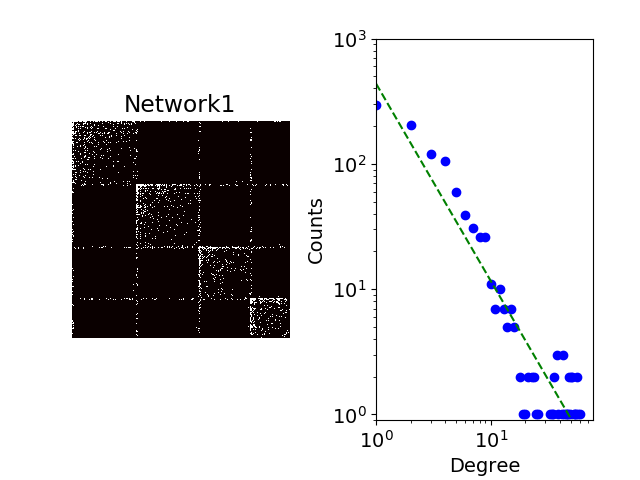
\includegraphics[width=1.1\textwidth]{img/corpus/network1_dd}
        \end{minipage}
        \begin{minipage}{0.35\textwidth}
            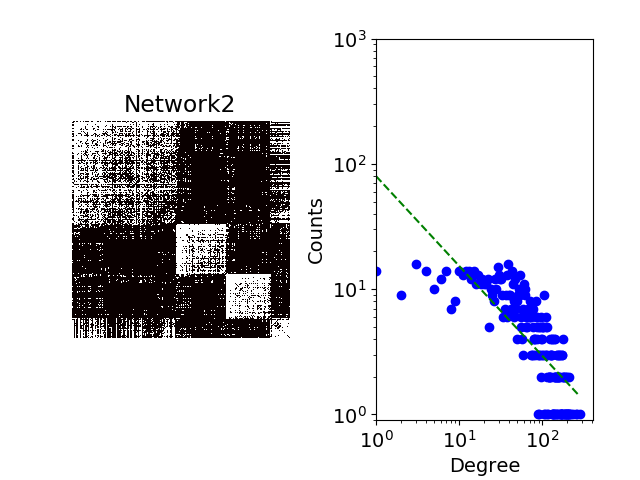
\includegraphics[width=1.1\textwidth]{img/corpus/network2_dd}
        \end{minipage}
        %\vskip\baselineskip
        \begin{minipage}{0.35\textwidth}
            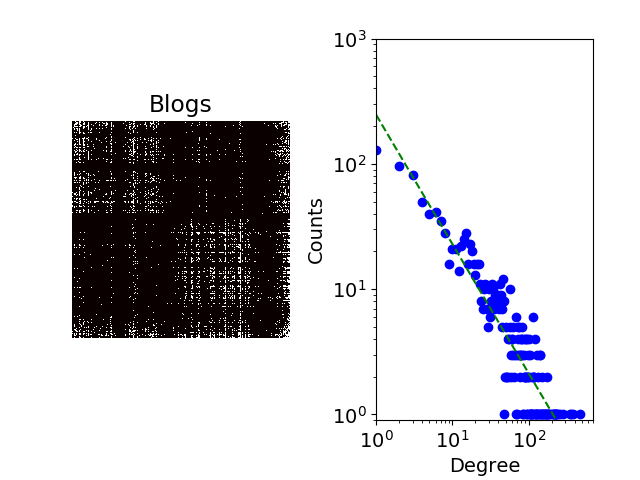
\includegraphics[width=1.1\textwidth]{img/corpus/blogs_dd}
        \end{minipage}
        \begin{minipage}{0.35\textwidth}
            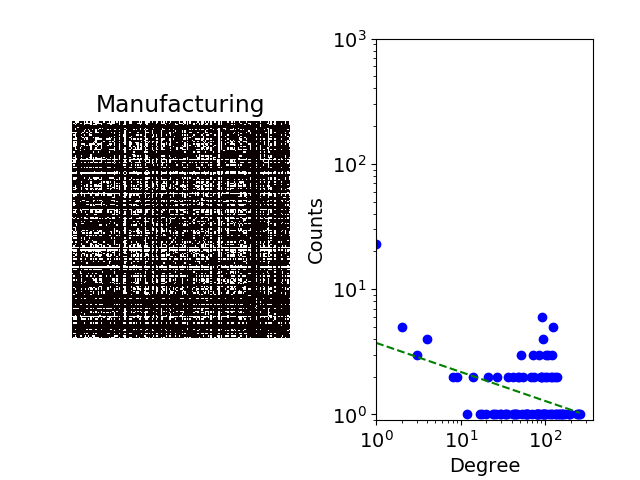
\includegraphics[width=1.1\textwidth]{img/corpus/manufacturing_dd}
        \end{minipage}
	\label{fig:corpuses}
\end{figure}


Pour chacun des jeux de données, nous avons inféré les paramètres des modèles \immsb~ et \ilfm  via des algorithmes de Markov Chain Monte Carlo (MCMC) sur 200 itérations. Pour \immsb, le paramètre de concentration du HDP a été optimisé en utilisant des priors gamma tel que $\alpha_0 \sim \text{Gamma}(1,1)$ et $\gamma \sim \text{Gamma}(1,1)$ en suivant la procédure de \cite{HDP}. Les paramètres de la matrice de poids $\lambda_0$ et $\lambda_1$ sont fixés à 0.1. Pour \ilfm, le paramètre $\sigma_w$ est fixé à 1 et le paramètre de concentration $\alpha$ de l'IBP fixé à 0.5 pour avoir une dynamique des classes comparable avec \immsb. Pour évaluer les distributions de degrés de ces modèles, nous générons un réseau complet (liens et non-liens) pour chaque n\oe{}ud du réseau source. Cette procédure est répétée 10 fois pour chaque expérience. Les valeurs des expériences pour la mesure des degrés des modèles  sont les moyennes et variances pour 10 répétitions indépendantes, présentées dans la Table \ref{table:me_gofit}. 
Il apparait que pour les modèles, l'attachement préférentiel global est uniquement vérifié sur les réseaux où la propriété était présente (Netwrok1 et Blogs) mais pas sur les autres, ce qui est en accord avec la proposition 3. Par ailleurs, dans le cas local, \immsb~ satisfait le test sur tous les réseaux avec de faibles fluctuations ce qui n'est pas le cas pour \ilfm~ pour qui les fluctuations sont plus grandes et surtout les paramètres de la loi de puissance sont très faibles. Ces faits confirment notre proposition 4.




\begin{table}[h]{Preferential attachment measures for training datasets and networks generated with fitted models.}
\begin{tabular}{lrrrr}
  \multirow{2}{*}{\textbf{Training Datasets}}  &
  \multicolumn{2}{c}{Global} & \multicolumn{2}{c}{Local}\\
  \cmidrule(r){2-3} \cmidrule(l){4-5}
  &   $p$-value &   $\alpha$   & $p$-value & $\alpha$   \\
\hline
Network1       & 1 & 2.4 &   1.0 $\pm$ 0.0  &  1.8 $\pm$ 0.03  \\
Network2       & 0 & 1.3 &   0.0 $\pm$ 0.0  &  1.2 $\pm$ 0.01 \\
Blogs          & 1 & 1.5 &   1.0 $\pm$ 0.0  &  1.4 $\pm$ 0.03\\
Manufacturing  & 0 & 1.4 &   0.4 $\pm$ 0.3  &  1.3 $\pm$ 0.05 \\
\hline

  \ \textbf{\immsb} &&&& \\
\hline
Network1       & 0.9 & 1.4 &   1.0 \(\pm\) 0.0   &  3.5 \(\pm\) 0.7 \\
Network2       & 0 & 1.3 &   0.9 \(\pm\) 0.0   &  1.6 \(\pm\) 0.2 \\
Blogs          & 1 & 1.3 &   1.0 \(\pm\) 0.0   &  4.3 \(\pm\) 1.1 \\
Manufacturing  & 0 & 1.2 &   0.9 \(\pm\) 0.01  &  1.6 \(\pm\) 0.1 \\
\hline

  \ \textbf{\ilfm} &&&& \\
\hline
Network1      & 1 & 1.4 &   1.0 \(\pm\) 0.0  &  1.7 \(\pm\) 0.1 \\
Network2      & 0 & 1.2 &   0.0 \(\pm\) 0.0 &  1.2 \(\pm\) 0.0 \\
Blogs         & 1 & 1.3 &   0.9 \(\pm\) 0.2  &  1.5 \(\pm\) 0.1 \\
Manufacturing & 0 & 1.2 &   0.3 \(\pm\) 0.3  &  1.3 \(\pm\) 0.0 \\
\hline
\end{tabular}
\label{table:me_gofit}
\end{table}


\begin{figure}[h] {Performance relative de \immsb\ and \ilfm\ en fonction de la proportion du jeux test.} 
        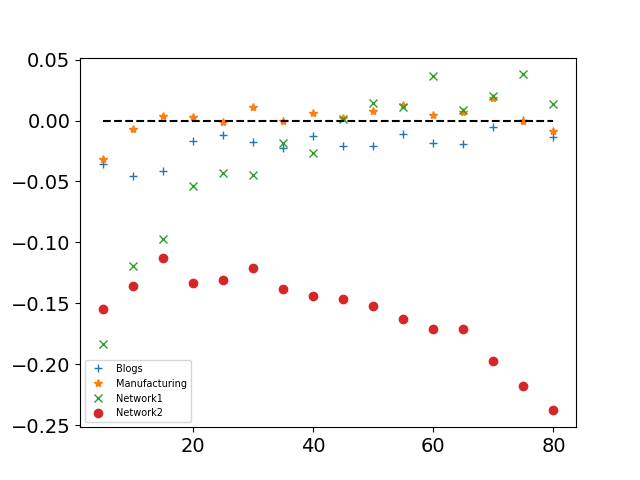
\includegraphics[scale=0.45]{img/corpus/testset_max_20.png}
\label{fig:auc}
\end{figure}

La figure \ref{fig:auc} propose une comparaison des modèles en fonction de la taille du réseau d'apprentissage, la comparaison correspond à la différence des valeurs AUC des deux modèles. Une ordonnée à 1 signifie que les deux modèles ont des performances identiques, et la zone au-dessus du 1 correspond à un avantage de \immsb~ sur ~\ilfm. Les abscisses correspondent à la proportion du nombre de liens non observés durant l'inférence. En général \ilfm~ obtient de meilleurs résultats que \immsb. Néanmoins la performance relative de ce dernier augmente quand le nombre de données d'apprentissage diminue sur les réseaux bursty, jusqu'a dépasser \ilfm. Alors que pour les réseaux non bursty c'est l'effet inverse qui est observé. Ce comportement illustre bien le fait que \immsb~ satisfait l'attachement préférentiel local, ce qui n'est pas vrai pour  \ilfm~ : quand les liens sont retirés aléatoirement, on a plus de chances de retirer des liens des classes les plus grosses que des petites; un modéle qui satisfait l'attachement préférentiel local à ainsi de meilleures chances de reconstruire ces classes altérées. A l'opposé, si la propriété n'est pas présente dans le réseau, un modèle qui la respecte sera pénalisé.

\section{Conclusion}

Nous avons étudié si les modèles \mmm, tel que \immsb~ et \ilfm, peuvent prédire des parties d'un réseau tout en satisfaisant les propriétés fréquemment observées dans les réseaux réels, à savoir l'attachement préférentiel et l'homophilie. Pour ce faire, nous avons introduit des définitions formelles de ces propriétés dans un cadre probabiliste et nous avons analysé comment se comportaient ces modèles au travers de ces définitions. Nous avons montré en particulier comment \immsb~ satisfait l'attachement préférentiel local. Ce résultat théorique a été validé expérimentalement sur des réseaux réels et synthétiques et permet de mettre en avant l'importance des propriétés inhérentes aux données pour choisir un modèle performant.












%\bibliographystyle{unsrt}
\bibliography{./a}

\end{document}
